\section{Execution}
\leavevmode\\
The execution of the models has been made with all the previous procedures regarding data processing in this paper. Data from subject 1 to 10 has been used to train the model, and data from 11 to 16 has been used to test the accuracy of the predictions of the model. For every file 50 epochs have been done to ensure a good understanding from the model of the data.
\\\\
At first the strategy of training and testing the model was done within the files of the subjects. For each file it was split in two by a percentage variable and afterword’s it was trained and tested. This strategy was abandoned because it wasn’t as efficient as if many files where trained, and afterwards tested for results. Because there are few seizures in the hole database it makes it difficult to train a model to understand the existence of a seizure. It was dependent on the position of data in the file, considering there a small amount, in most cases only one seizure per file, if the file was split one half would have a seizure and the other would not have one. This is a big problem if training has no seizure and the testing data has it. It would never be able to learn what a seizure is. Opposite to the previous statement, it might learn what a seizure is, but it would never be possible to test it, if it learned correctly to classify.

\leavevmode\\
\begin{figure}[h!]
  \caption{Data from subject 12 file 8 seen scattered through the hole recording}
  \centering
  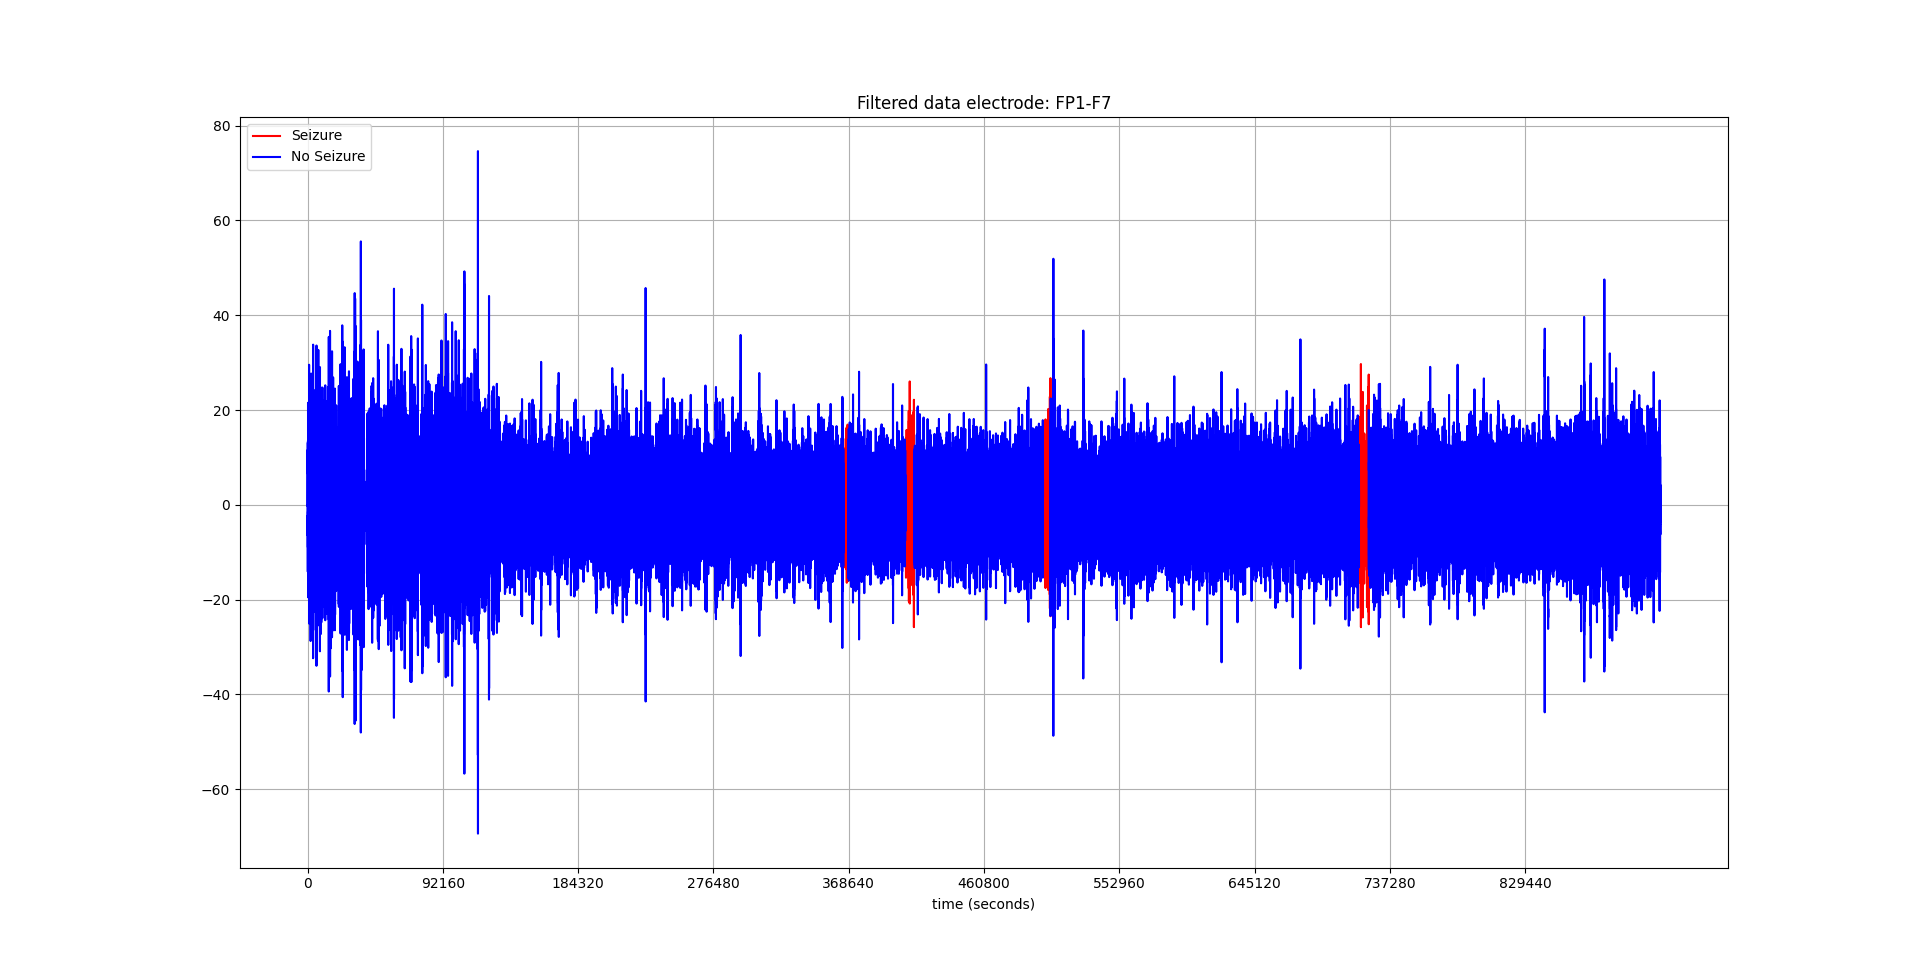
\includegraphics[width=0.5\textwidth]{img/12_8-elecFP1-F7.png}
\end{figure}

\begin{figure}[h!]
  \caption{Data from subject 1 file 3 with only one seizure. This file wouldn't be eligible to split in train and test }
  \centering
  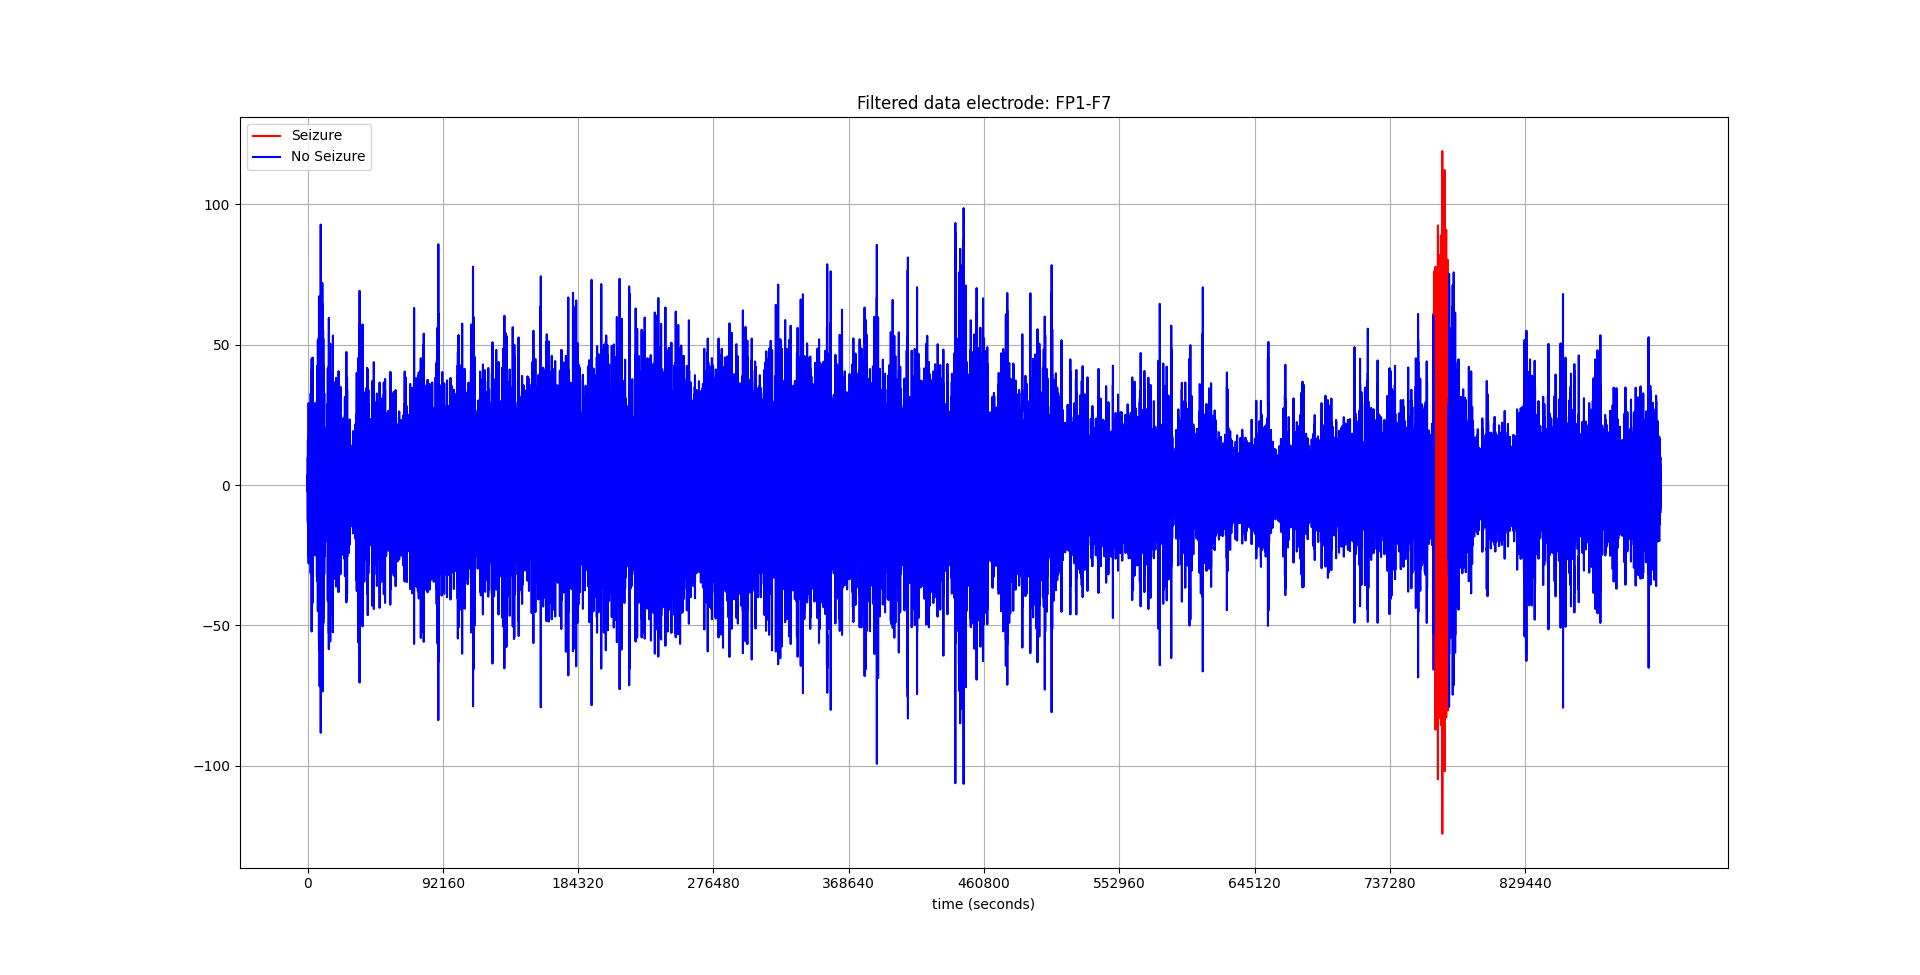
\includegraphics[width=0.5\textwidth]{img/1_3-elecFP1-F7.png}
\end{figure}
\leavevmode\\
In the end the strategy of first training the model with some files and then with others do the testing, was the best strategy, considering training each file took around 10 minutes depending on the computer it was executed with. There was a big difference between executing the model with and without Cuda. The first model CNN\_ConcatInput, was executed without Cuda because of the hardware architecture. It spent around 30 hours training the model. The second model CNN\_ProjOut\_Conv, was executed with Cuda and spent training around 15 hours. It is important to consider using a desktop computer to train the model, considering it will get hot finishing the last epochs of every file.
\\\\
Executing this type of models is also very resource consuming, considering it loads all the file to RAM to read and work with it from there. It could be a problem to many computers, because the ones with 8Gb will not work. Only with 16Gb of memory worked for me. In most cases, the edf files contains exactly one hour of digitized EEG signals, although those belonging to case chb10 are two hours long, and those belonging to cases chb04, chb06, chb07, chb09, and chb23 are four hours long; occasionally, files in which seizures are recorded are shorter, so the idea of concatenating files of a subject to have one file per subject it is also excluded.
\\


\section{Conclusion}
\subsection{Results}
\leavevmode\\
After training the two models with files from subjects 1 to 10, testing only took 15 to 30 minutes to execute with subjects from 11 to 16. The results given by the function classification\_report of the library metrics from sklearn were saved in parquets and then loaded with the “05\_ReadParquet.py” script. This script reads every parquet from the folder results of every tested subject and displays the results on the terminal. 
\\\\
At first results looked promising viewing a staggering 95\% to 100\% accuracy in classification from the model. But upon further inspection the results are bad, because I realized the accuracy given by the report was because it predicted all data to be “no seizure”. The other 5\% is the Seizure in the data that the model is classifying it was no-seizure. Because data is mainly one-sided to no-seizure, the result 95\% is because it was only classifying this class. In the end, it is returning the percentage of the amount of data of each class.
\\\\
Looking up the results and the model, I realized the data in the input of the model is not exactly as expected. There are inconsistencies in the results, for example as shown in the next two tables, these should have the same dimensions but here it is not the case:
\leavevmode\\

\begin{table}[H]
    \caption{Results from subject chb14 file 6}
    \begin{tabularx}{\columnwidth}{ @{\extracolsep{\fill}} |c|c|c|c|}
        \hline
                        & \textbf{0} & \textbf{1}                 & \textbf{accuracy} \\ \hline
        \textbf{precision} & 0.983      & {\color[HTML]{FE0000} 0.0} & 0.983             \\ \hline
        \textbf{recall}    & 1.000      & {\color[HTML]{FE0000} 0.0} & 0.994             \\ \hline
        \textbf{f1-score}  & 0.997      & {\color[HTML]{FE0000} 0.0} & 0.994             \\ \hline
        \textbf{support}   & 358.00     & 2.0                        & 0.994             \\ \hline
    \end{tabularx}
\end{table}

\begin{table}[H]
    \centering
    \caption{Results from subject chb14 file 11}
    \begin{tabular}{|l|l|l|}
        \hline
                        & \textbf{0} & \textbf{accuracy} \\ \hline
        \textbf{precision} & 1.0        & 1.0               \\ \hline
        \textbf{f1-score}  & 1.0        & 1.0               \\ \hline
        \textbf{support}   & 360.0      & 1.0               \\ \hline
    \end{tabular}
\end{table}
\leavevmode\\
The two tables are from the same subject. These represent the results of testing files chb14\_06 and chb14\_11. Both tables are from are from the same subject 14. These should have the same size of dimensions in columns, defined by 22 electrodes plus the seizure’s column and the windows column. The second dimension could change from file to file, because of the interruptions while recording as explained previously in this paper. The reason why the tables are different, one of them lacking from having the class 1 (class seizure, marked in red in the table), it is because when testing the model did not recognize a class as such. In further inspections surprisingly the data was only represented by one class, and as explained earlier, all files fed to the model where files with one or more seizures in them. All reports of testing should have strictly columns 0 and 1.
\\\\
This problem is obviously an issue regarding data processing. Some files seem to be having problems with the dimensions of the numpy array. It seems to be working fine up until the labelling of the data. Once is read from the parquet and the data is set with the windows, then some problems seem to appear on the dimensions of the windows. I think the problem is on the equation regarding the overlapping and window sizing.
\\\\
The size of the windows is set by a variable in a common dictionary with all the data processing characteristics needed to run the script, as well as the overlap. The size of the window is set for the model to be able to work within this window and not with the hole file, as it would be very resource intensive to execute and not as efficient to train. The size of the window is defined by a constant, in this case is set to 10 seconds, because generally, working with seizures the range of the window’s size is around 5 seconds to 10 seconds. The equation could be having issues setting the values correctly, because depending on the length of the recording, some files have issues with this matter. In conclusion, the model is not receiving the data as it should.
\leavevmode\\


\subsection{Future Work}
For future work it would be strictly necessary first of all, to change the chunker function setting the windows of all the files. Assuming the model works as it should, getting the right processed data would be enough to have a consistent result. If the result of the classification is not good enough, I would consider adding a weighted cross entropy loss to avoid so much one-sided data, for the model to learn more uniformly.
\\\\
When training and testing the model, it would be a good idea to only do these two procedures. A good way to avoid extending training and testing execution time would be to normalize data before any model execution. This way all files, would be normalized considering all files and not just only one, like it is done in the execution script. As previously mentioned, the scalers are obtained by only considering one file. An average of scalers should be considered to keep in touch with the type of signals of every file, especially normalizing data between subjects, because seizure characteristics could change between different subjects, having a different impact on the model.
\\\\
With better results the difference between models could be further proven, to understand the best strategy to obtain and process data. Not only two models, but all the models offered by the CVC (CNN\_ConcatInput, CNN\_ProjOut\_Conv, CNN\_ProjOut\_Concat, CNN\_ProjOut\_AvgW, CNN\_ProjChannel, CNN\_ProjChannel\_v2, Seq\_C1D, Seq\_C1D\_Ensemble).
\\\\
Regarding biological characteristics, other models that consider data sequences could be also utilised such as Dominant Sequence Transduction models, like states Attention is All you Need paper. Creating a model and maybe consider classifying data in three classes: seizure, no seizure and pre-seizure. This would enable people to predict seizures and further understand the reason of them if these are linked to a sequence or pattern. This type of algorithm is used to understand sequences, such as natural language processing. If the existence of seizures is linked to a history of patterns that could be recorded in encephalograms and processed to predict when it is likely to be another seizure. Models could be trained and future devises could be programmed and created to at least advice or warn the subject a seizure is about to appear. Other problems could be avoided because the subjects could brace themselves, and take precautions such as seating down, closing the mouth, or simply get in a position more secure before the seizure happens.
\\\\
Data processing with other ranges of frequencies would be another issue of research as well, because in this paper only theta frequencies are considered and all other excluded, but there’s also delta, alpha, beta, gamma to research with, and it would be interesting to find out if a model could learn better from other bandwidths, and classify which one’s are better for classifying seizures.
\\\\
The position of the electrodes has been taken care of in the processing script, in a way where if there is an interruption and electrodes are changed, then the file was automatically excluded. But this could be changed to match the data of the previous positions of the electrodes and the positions of the one’s after the interruption. This way more data could be used to train the models as well as maybe considering different Brodmann’s areas (explained in the annex), to give more importance to data coming from certain areas in the brain which could cause or give more information about the reason, detonation or existence of seizures.
\\\\
As this paper the model was trained with different subjects because there’s not enough data to train with, it should be considered if different people have the same “type of seizure” affecting in the learning of the model. If enough data from only one subject was enough to train the model, it should be considered if this model could also predict seizures in other subjects with the same problem. The seizure itself might change between subjects, so maybe it’s alright to train the model for now with different subjects to consider many possibilities. 
\\\\
Finally other datasets should be researched as well to have a big overview of the difference in data between datasets regarding the seizure issue. It’s hard to come by with any, but it could help a lot with the learning of models to find out how seizures come to be. Also, other scripts should be created to process data for the model to input the same way, with the same characteristics, as it’s done with this dataset. For sure, this would be much more time consuming but with promising results.
\\

\section{Acknowledgments}
\leavevmode\\
In the production of this TFG there has been a lot of people involved helping me to make this project as it is right now. When I first started working with Aura Hernandez and Debora Gil, they provided me with the code of the models to change and adapt to the dataset CHB-MIT I have been working with in this TFG. Because this team is working on the Mental Workload Detection, they provided me with all sorts of scripts in models and data processing. I was able to make an idea of what I wanted, but because of the big difference on the datasets, data processing scripts had to be redone completely as well as modifying the models to fit and work with the new database.
\\\\
Once I was working with this TFG, mid-way I started to have problems with my lack of knowledge on how torch works. I desperately needed an in-depth insight on how the models were created and the reason of the internal structure. With Jose Elias we have been doing all kind of reunions to further understand these issues and also consider other strategies on how to process data more efficiently. Being able to work with someone who already has experience in this field of artificial intelligence has given a boost with the development of this project my own personal knowledge.
\\\\
I would like to consider the effectiveness in response from Jordi Pons when there’s a problem or simply any doubt. It’s someone to surely rely on, he’s always around and willing to help, this attitude is well known and appreciated by all.
\\\\
Last but not list, special thanks to my teacher Aura Hernandez helping me review, schedule and manage this project as important as it is. Training models, providing information and guidance on any topic, followed by a big interest in the subject and charisma, makes difficult times easier to overcome.
\\\\
Much appreciated everyone who has showed interest in this project. I wouldn’t have done it without the help of all professionals involved in this project, thank you all.
\\